\comment{
\jpginput{}{led-array}{}
\jpginput{}{myholo}{}
\jpginput{}{phase}{}
\jpginput{}{tf-gpc}{}
\jpginput{}{dunsby}{}
\jpginput{}{aod}{}
}

\chapter{Other approaches of light control}
\label{sec:approaches}
\nomenclature{CLEM}{Controlled light exposure microscopy}%
\begin{summary}
  This chapter gives an overview of current microscopy techniques that
  reduce unnecessary fluorescence excitation and reduce
  phototoxicity. In \emph{light sheet microscopy}, an oblique sheet of
  light illuminates the sample without exposing too many out-of-focus
  fluorophores. \emph{Controlled light exposure microscopy} (CLEM)
  takes into account the in-focus fluorophore distribution and
  iteratively improves the signal-to-noise ratio of the measurement.
  Finally, \emph{light field microscopy} allows instantaneous and
  complete control of all parameters of the incoherent light exposure.
\end{summary}
\section{Light sheet fluorescence microscopy}
\label{sec:light-sheet-microscopy}
\begin{summary}
  Light sheets can be directly created with separate optics to
  illuminate the sample from an orthogonal direction. Another
  promising method to create a sheet is to use a high numerical
  aperture objective near the total internal reflection
  angle. Diffraction couples the minimum width of the sheet and the
  extent of the area, where the sheet's width is constant. There is a
  trade-off between sheet width and field of view.
\end{summary}
The idea of illuminating a sample from the side dates back quite far
into the history of microscopy. Already one hundred years ago, an
additional objective, arranged perpendicular to the detection
objective, was used for illumination of the focal plane in the
specimen. This dark field technique was used to characterize gold nano
particles in gold ruby glass \citep{Siedentopf1903}.

Eventually, this illumination method was also applied for fluorescence
microscopy. First, to analyze cochlea specimen \citep{Voie1993} and,
more recently, for the development of embryos
\citep{Huisken2004}. Results in the latter paper have sparked interest
in the technique at many labs \citep{Santi2011}.
\subsection{Light sheet generation with cylindrical lens}
\begin{figure}[!hbt]
  \centering
  \svginput{1}{spim-sketch}
  \caption{Schematic of SPIM (selective plane illumination
    microscope). A cylindrical lens illuminates the specimen with a
    thin sheet of light along the focal plane of the
    objective. Rotating the sample and/or moving it along the axis
    allows to reconstruct a sectioned three-dimensional volume of the
    fluorophore concentration with improved light utilization compared
    to conventional microscopes \citep[inspired from][]{Huisken2004}.}
  \label{fig:spim}
\end{figure}
\figref{fig:spim} shows how the light sheet can be focused into the
specimen using a cylindrical lens. \cite{Huisken2004} employ a water
dipping objective with long working distance (\unit[1\ldots 2]{mm})
and comparatively low NA for detection. A $10\times$ objective with
$\unit[660]{\mu m}$ field of view diameter is used with a sheet
thickness that varies less than $42\%$ ($\unit[6\ldots 8]{\mu
  m}$). The light sheet not only improves sectioning and contrast but
also increases the axial resolution from originally $\unit[14]{\mu m}$
by nearly a factor of two.

\nomenclature{SPIM}{Selective plane illumination microscopy}

The axial resolution of detection objectives with higher numerical
aperture isn't improved so easily over an extended field of
view. Shading effects, diffraction and refraction can deteriorate the
light sheet. As an improvement of the technique it was suggested to
rotate the specimen or illuminate with multiple sheets of light from
different directions.

A major difference between this technique and more conventional
microscopy techniques is the way the sample is mounted. In a normal
microscope, usually, a specimen is placed with a drop of embedding
medium on a \unit[170]{$\mu$m} thick cover slip. Then it is flipped
onto a microscope slide and sealed with nail varnish. This approach of
mounting the sample does not work for an ultramicroscope because there
the sample has to be accessed from two perpendicular sides. Often the
specimen are embedded in an agarose cylinder or sometimes, they are
fixed in a liquid--filled chamber.

\subsection{Light sheet generation using the detection objective}
\label{sec:hilo}
\begin{figure}[!hbt]
  \centering
  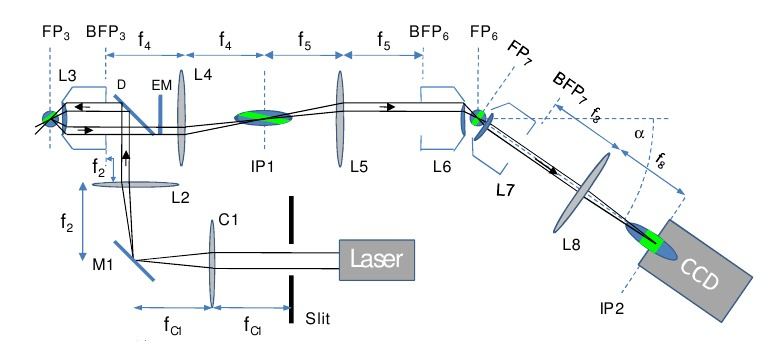
\includegraphics[width=12cm]{dunsby}
  \caption{Schematic of oblique plane microscopy (OPM). An index
    matched sample is excited using an oblique plane of light. The
    illuminated plane is tilted relative to the focal
    plane. Therefore, out-of-focus fluorophores on the periphery of
    the field of view are excited as well. Two additional objectives
    in the detection path are used to reconstruct an aberration free
    image of all the excited fluorophores (drawing from
    \cite{Dunsby2008}).}
  \label{fig:dunsby}
\end{figure}
Modern high numerical aperture objectives allow to illuminate an
\emph{index matched} sample with a half angle of up to
$70^\circ$. This enables illumination of an oblique and thin sheet of
light in the specimen just as in selective plane illumination
microscopy. However this technique (oblique plane microscopy, OPM) has
the advantage, that only one objective is and therefore it will work
with conventional microscope slides. However, one difficulty is that
some of the excited fluorophores are severely defocused in the
intermediate image plane (see plane IP1 in
\figref{fig:dunsby}). Dunsby describes how to rotate the observational
plane optically in order to recover an aplanatic image from the
oblique illumination plane \citep{Dunsby2008}. They re-image the
sample through two additional objectives.

\nomenclature{OPM}{Oblique plane microscopy}

\begin{figure}[!hbt]
  \centering
  \svginput{1}{hilo-sketch}
  \caption{Schematic of rays in HILO (highly inclined and laminated
    optical sheet) technique. The specimen is embedded in a medium of
    lower optical density than the cover slip. For a very high
    illumination angle (point on the periphery of the back focal
    plane), the light would be reflected at the cover slip-medium
    interface due to total internal reflection. For HILO, a point on
    the back focal plane that is closer to the optic axis is
    illuminated. The light enters the embedding medium at a highly
    inclined angle and only a thin sheet in the focal plane is
    illuminated \citep[inspired from][]{Tokunaga2008}.}
  \label{fig:hilo}
\end{figure}

Biological specimen are often not index matched and have a lower index
$n_e\approx 1.33\ldots1.45$ than the immersion oil $n=1.52$. As
indicated in \figref{fig:hilo}, the refraction at the interface
between cover slip glass and embedding medium can be exploited to
illuminate the specimen with a light sheet that is nearly parallel to
the focal plane.  This technique is called highly inclined and
laminated optical sheet microscopy (HILO) \citep{Tokunaga2008,
  Konopka2008}.

\nomenclature{HILO}{Highly inclined and laminated optical sheet microscopy}

Note that the index mismatch between embedding and immersion medium
will introduce aberrations (mostly spherical) in the detection which
will limit the useful imaging depth to a few microns for high aperture
lenses.
\section{Scanning techniques for improving light utilization}
\begin{summary}
  In section \ref{sec:2-photon} we already introduced the 2-photon
  microscope. Its phototoxicity and speed can be improved with the
  methods that are described in the following two subsections.
\end{summary}
\subsection{Controlled light exposure microscopy (CLEM)}
\label{sec:CLEM}
The confocal microscope (see \figref{fig:widefield-microscope}~c)
allows another adaptive illumination technique. Each point in the
focal plane of the specimen is treated as one of the following three
cases: point with no fluorophores (A), high concentration of
fluorophores (C) or an intermediate (B).

Ideally, points of type (A) that do not contain fluorophores should
only be exposed until fluorophore content is ruled out. The other two
classes (B) and (C) should be exposed until a fixed number of
fluorescence photons have been detected (C) or a maximum integration
time has been reached (B). Unfortunately, due to the photon nature of
light, sometimes a region of type (B) is incorrectly treated as (A)
which introduces dark pixel artifacts in the image
\citep{Hoebe2010}.

In conventional microscopes, areas of class (C) with high fluorophore
concentration are generally exposed too much. Their signal-to-noise
ratio would be high, but this doesn't increase the perceived image
quality. Furthermore, the regions above and below the focal plane are
unnecessarily subjected to high exposure.

The CLEM approach was first presented by Hoebe et al.\ in
2007,\todo{was that first, get}\ followed by an independent similar
version with adaptive control of the laser power for 2-photon
microscopy by Chu et al.\ \citep{Hoebe2007,Chu2007}.
\subsection{Acousto-optic deflectors for fast beam steering}
In a conventional confocal microscope, the beam is steered by two
galvanometer mirrors. This technique offers very good light throughput
and is sufficient to obtain rectangular images. However, the inertia
of the mirrors severely limit the access rate of spots in the focal
plane.

Replacing the mechanical mirrors with an acoustic wave in a
transparent material (TeO$_2$) enables $\unit[4]{\mu s}$ switching
time \citep{Otsu2008} and even allows re-focusing
\citep{Reddy2008}. These acousto-optic deflectors have lower
efficiency than mirrors (70\% for two AODs) and show chromatic
aberrations.

However, as descanning isn't necessary in 2-photon microscopy, the
lower efficiency (in the excitation path) is hardly an
issue. Therefore, this technique for the first time enables ``random
access'' of three-dimensional coordinates in the sample.

\begin{figure}[!htbp]
  \centering
  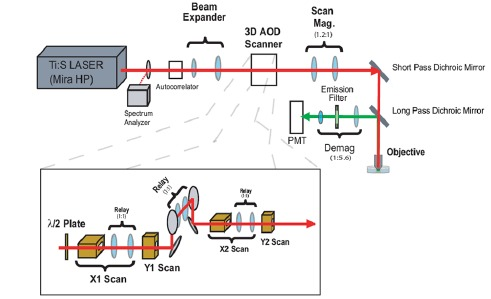
\includegraphics[width=12cm]{aod} 
  \caption{Schematic of an acousto-optic deflector (AOD) illumination
    system with $z-$focusing. Figure taken from \citet{Reddy2008}}
% in focusing single s highly preferred http://www.future-perfect.co.uk/grammartips/grammar-tip-focussed-focused.asp
  \label{fig:aod}
\end{figure}


\nomenclature{AOD}{Acousto-optic deflector}
\nomenclature{AOM}{Acousto-optic modulator}

% FIXME
\cite{botcherby2012aberration}


\section{Non-scanning techniques}
\subsection{Direct illumination}
An obvious method for doing spatial control is to image a
two-dimensional array of high-power micro-LEDs into the specimen.
\begin{figure}[!hbt]
  \centering
  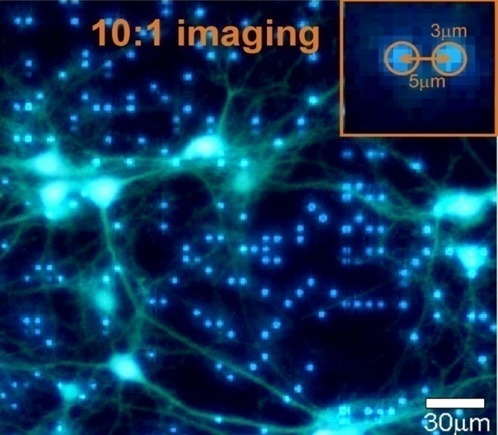
\includegraphics[width=7cm]{led-array} 
  \caption{An overlay combining wide field micro-LED illumination and
    fluorescence imaging YFP tag expressed in neurons, taken from
    \citet{grossman2010}.}
  \label{fig:led-array}
\end{figure}
However, the problem is to achieve sufficient \emph{irradiance} and
\emph{fill factor}. The angular emission profile of LEDs is often
Lambertian, i.e.\ the back focal plane of the objective would be
over-illuminated and a lot of light would be lost. The fill factor is
limited because it is difficult to put a lot of LEDs close to each
other.  The technique has been demonstrated using a $64\times64$ array
of $\unit[20]{\mu m}$ micro-emitters with $\unit[50]{\mu m}$ pitch
\citep{grossman2010}.  The LEDs can be switched at millisecond speed
and emit at $\unit[(470\pm22)]{nm}$.

\nomenclature{GFP}{Green fluorescent protein}
\nomenclature{EGFP}{Enhanced green fluorescent protein}
\nomenclature{YFP}{Yellow fluorescent protein}
\nomenclature{VCSEL}{Vertical-cavity surface-emitting laser}
\nomenclature{LED}{Light-emitting diode}
\nomenclature{MMA}{micro-mirror array}
\nomenclature{LCoS}{Liquid crystal on silicon (display)}
\nomenclature{DPSS}{Diode-pumped solid-state (laser)}

LED arrays enable interesting experiments where processes are
influenced by light, i.e.\ optogenetics, but the targets ideally have
to be located in the focal plane. Also, it must be verified that the
illumination cone of each LED image doesn't affect the measurement,
i.e.\ activate the specimen in the out-of-focus regions.

Nevertheless, once the LED or VCSEL arrays become available in
interesting spectral ranges, we might see the direct illumination
techniques more often.

\subsection{Intensity modulation}
\subsubsection{Programmable array microscopy}
A technique similar to controlled light exposure microscopy (CLEM,
section \ref{sec:CLEM}) has been implemented in a programmable array
microscope (PAM) \citep{Caarls2011}. Like our microscope, the PAM
images a pattern into the sample using a spatial light
modulator. Contrary to our system, the same SLM is used in the
detection path to recover an image of the in-focus fluorophores.

\begin{figure}[!hbt]
  \centering
  \svginput{1}{pam-sketch}
  \caption{Schematic of a programmable array microscope (PAM)
    \citep[inspired from][]{Verveer1998}. A digital micromirror
    device (DMD) containing an array of tiltable mirrors is imaged
    into the focal plane of the objective. Returning fluorescent light
    from out-of-focus fluorophores is distributed onto both the
    cameras. In-focus fluorescence is only imaged onto camera 1.}
  \label{fig:pam-sketch}
\end{figure}


\nomenclature{PAM}{Programmable array microscopy}%
\nomenclature{DMD}{Digital micro mirror device}%
\nomenclature{MLE-PAM}{Minimized light exposure programmable array microscope}%

\subsubsection{Light field microscopy}
\label{sec:light-field-microscopy}
Interesting work on light fields originally started in the macroscopic
domain of cameras \citep{Lippmann1908%,Sokolov1911
} and was eventually applied as a technique for microscopy
\citep{Levoy2006,Levoy2009,Zhang2009}. This approach is built on
imaging through an array of microlenses.
\begin{figure}[!hbt]
  \centering
  %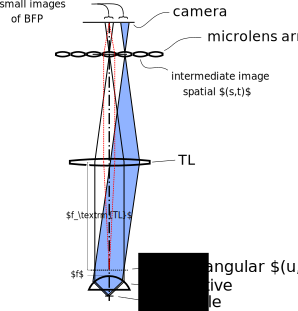
\includegraphics[width=7cm]{microlens-levoy-sketch} %FIXME redraw
  \svginput{1}{microlens-levoy-sketch}
  \caption{Schematic of microlenses in intermediate image plane
    \citep[inspired from][]{Levoy2006}}
  \label{fig:microlens-levoy-sketch}
\end{figure}

A microlens array is placed behind the intermediate image plane (see
\figref{fig:microlens-levoy-sketch}). The light that illuminates one
microlens corresponds to one spot in the focal plane of the
sample. The camera is positioned in the focal plane of the microlenses
and captures an image of the back focal plane behind each microlens
(see red ray bundle in \figref{fig:microlens-levoy-sketch}).

The camera captures the four dimensional light field, leaving the
specimen with spatial coordinates $(s,t)$ and angular coordinates
$(u,v)$. This data enables computational viewpoint shifting,
refocusing, extended depth of field and aberration correction of the
detected fluorescence emission.

\begin{figure}[htbp]
  \centering
  \svginput{1}{microlens-levoy-sketch_2}
  \caption{Construction of an out-of-focus ray bundle through the
    light field microscope. In order to improve the readability of the
    drawing, the magnification in the microscope was set to $1:1$
    (focal lengths of tube lens and objective are equal). An on-axis
    sample point originating from below the focal plane of the
    objective is imaged onto an on-axis point between the tube lens
    and the microlens array. Three of the microlenses re-image this
    on-axis image point into three points behind the plane of the
    camera, i.e.\ the images behind the three microlenses will contain
    bright blurry spots at different positions relative to their
    centre.}
  \label{fig:microlens-levoy-sketch_2}
\end{figure}

\figref{fig:microlens-levoy-sketch_2} shows a bundle of rays
originating from an out-of-focus point. Each of the microlenses that
are hit by the circle of confusion, re-image a fraction of the angular
range into a small image.  This process is crucial because a lot of
the original image information is lost here. The intensities from the
sub-images on the camera can't later be recombined in order to, say,
recover a high resolution image of the defocused point
\citetext{priv.\ comm.\ R.~Heintzmann}.

Additionally the light field microscope doesn't utilize the full
resolution of high-NA objectives. This will prevent the use of this
technique in its current form in the detection path of microscopes.
When the microlenses are small enough, to obtain a high resolution
image of the sample, then the angular resolution diminishes.

However, the same idea can be applied in the excitation path
\citep{Levoy2009}. For illumination purposes, lower resolution will
often suffice. The light-field technique allows unique control of
excitation light intensity and angles at each point of the sample
plane.

\nomenclature{TL}{tube lens}
\subsection{Temporal focusing}
\begin{figure}[!hbt]
  \centering
  \svginput{1}{temporal-focus-sketch}
  \caption{Schematic of temporal focusing \citep[inspired
    from][]{Oron2005}. A grating in the intermediate image plane
    separates the pulse into its spectral components. The out-of-focus
    areas of the specimen are illuminated with a longer pulse. Only in
    the focal plane, all spectral components interfere coherently and
    form a short intensive pulse.}
  \label{fig:oron}
\end{figure}
The axial extent of ultra-short laser pulses can be as thin as a few
microns. A parallel beam can be split into different spectral
components by a grating in the intermediate image plane
\citep{Oron2005}. The tube lens focuses the diffraction pattern into a
line in the back focal plane of the objective.

The objective, which has to be corrected for chromatic aberration and
dispersion, then focuses all the beams onto the focal plane. Different
spectral components arrive in the focal plane at the same time. The
out-of-focus points see an extended illumination. For a high NA
objective, a pulse duration of $\tau=\unit[20]{fs}$ results in slice
of $z\approx\tau c/2\approx\unit[3]{\mu m}$ thickness around the
focus, where the beam has significant intensity.

Using this technique it is possible to build a wide field 2-photon
microscope. That only excites fluorophores within the focal plane. The
technique can be further improved by spatially modulating the beam in
the intermediate image plane for CLEM like performance. This technique
has been implemented in the TF-GPC approach and will be discussed in
the next section.

\subsection{Phase modulation}
\subsubsection{Digital holography}
\begin{figure}[!hbt]
  \centering
  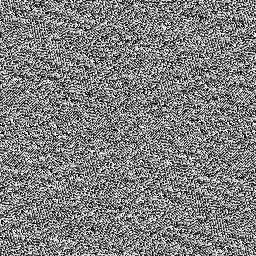
\includegraphics{myholo}\quad
  \svginput{1}{phase-holo_my} 
  \caption{Schematic of spatial illumination by phase holography. A
    phase-only SLM displays a hologram in the plane $P'$ which is
    conjugated to the back focal plane $P$ of the objective
    \citetext{inspired by slide from V. Emiliani}.}
  \label{fig:phase-holo}
\end{figure}
Certain types of liquid crystal spatial light modulators can be used
to modify the phase of light. When such a device is placed into the
back focal plane of a lens, it is possible to control the light
distribution in its front focal plane. An iterative algorithm
(iterative Fourier transform algorithm, IFTA) can be used to establish
a phase image on the liquid crystal display that will result in an
intensity distribution in front of the lens.

\nomenclature{IFTA}{Iterative Fourier transform algorithm}

This approach has been used to excite a two-dimensional pattern in the
specimen \citep{Lutz2008,Zahid2010} and is advantageous especially for
cases where only small parts of the specimen ought to be
illuminated. As opposed to conventional intensity spatial light
modulators, the light can be redirected from dark areas into the
bright areas.

% single photon 405nm uncaging, ifta,
% spherical wave approximation
There is also a limited possibility to create three-dimensional
patterns, e.g.\ several points below, in and above the focal plane by
displaying Fresnel zone planes.  For illumination, usually a laser
with non-zero interference length is employed. However, this
illumination contains an unwanted ``speckle'' pattern in the form of
noisy non-uniformities. To a certain extent, the contrast of the
speckle pattern can be reduced by controlling spatial and temporal
coherence of the illumination (sweeping the frequency of the laser or
changing illumination direction while the detector is integrating).

Holographic control can be used with 2-photon excitation as well
\citep{Nikolenko2008}, % two photon
but this exacerbates the effect of speckles.
\subsubsection{Generalized phase contrast (GPC)}
\begin{figure}[!hbt]
  \centering
  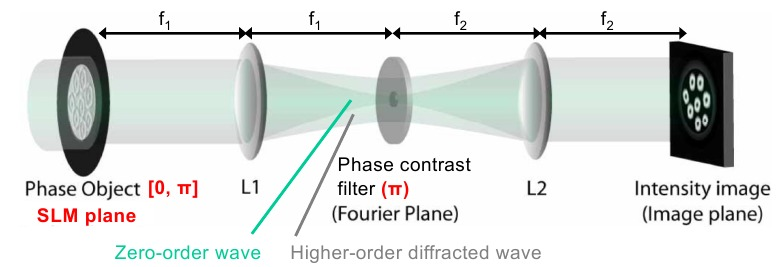
\includegraphics[width=14cm]{phase} % FIXME redraw
  \caption{Schematic of generalized phase contrast
    \citep[from][]{Rodrigo2008}.}
  \label{fig:phase}
\end{figure}
A phase contrast microscope objective \todo{modified ?} can be used to
convert a phase image from the intermediate image plane into an
intensity image in the specimen \citep{Rodrigo2008}\todo{read more of
  this}. Compared to digital holography, hardly any computation is
necessary. Yet, the phase spatial light modulator allows to
concentrate a lot of light even on a small region of the specimen as
opposed to other techniques, which involve intensity modulation and
lose all the light of dark areas by sending it into a beam block or
something similar.

The generalized phase contrast method is suitable even with spatially
incoherent illumination\todo{slightly ?}. However, when the
fill-factor -- the size of the bright area in the image -- changes,
the phase contrast filter must be changed.
\subsubsection{Generalized phase contrast and temporal focusing (TF-GPC)}
The combination of generalized phase contrast and temporal focusing
allows spatially controlled illumination of in-focus areas
\citep{Papagiakoumou2010}. Usage of a phase spatial light modulator
results in high light efficiency compared to intensity modulation.
Splitting and recombination of the spectral components of the pulse
reduce speckle noise considerably.
\begin{figure}[!hbt]
  \centering
  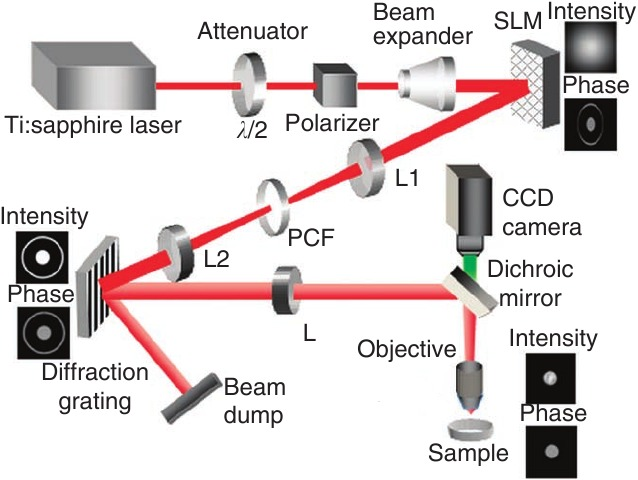
\includegraphics[width=11cm]{tf-gpc} 
  \caption{Schematic of phase contrast with temporal focusing (TF-GPC)
    \citep[from][]{Papagiakoumou2010}, PCF is a phase contrast filter.}
  \label{fig:tf-gpc}
\end{figure}
\nomenclature{PCF}{Phase contrast filter}

%%% Local Variables: 
%%% mode: latex
%%% TeX-master: "kielhorn_memi"
%%% End: 
